% Part 1: Detecting DNA-bound RecB molecules
\section*{Results}

\subsection*{Imaging DNA-bound RecB molecules}

\begin{figure*}[htbp]
    \centering
    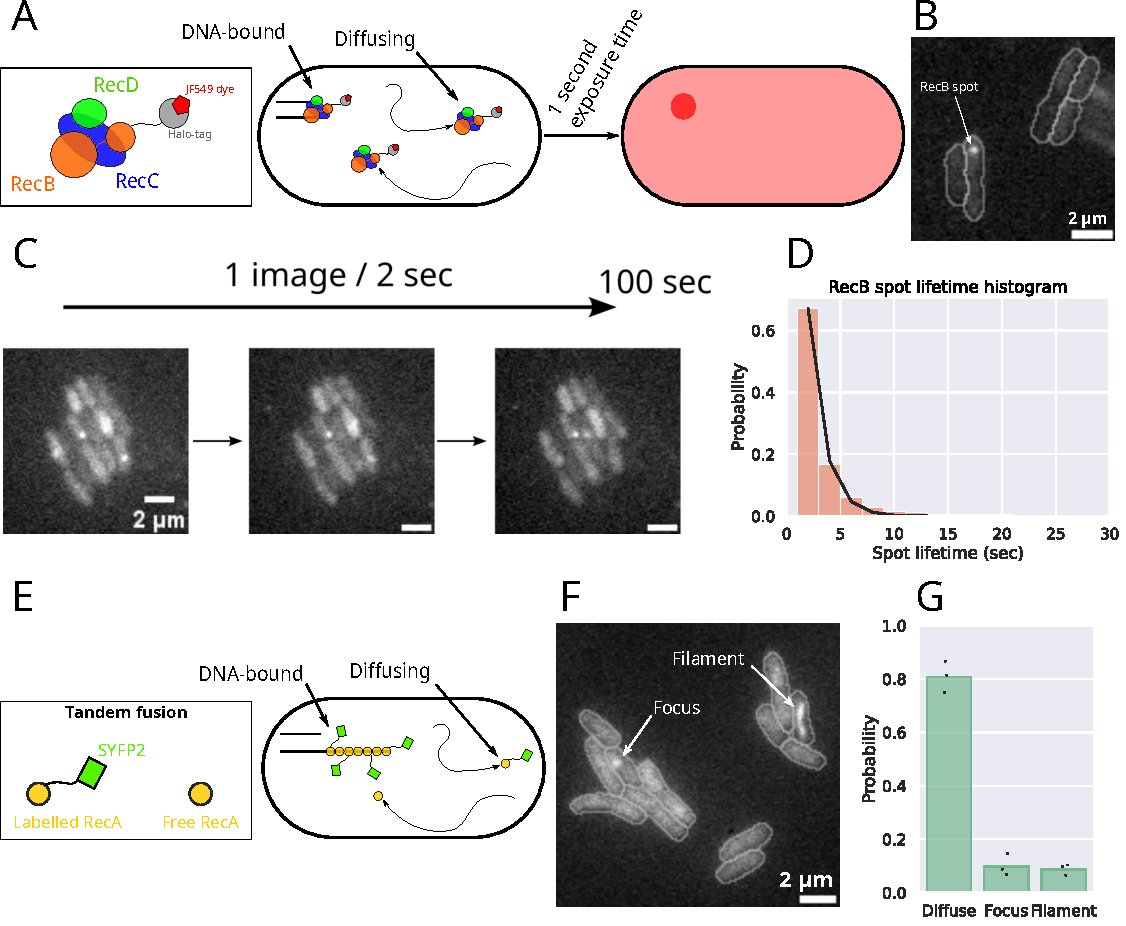
\includegraphics[width=.8\textwidth]{Figures/Fig1_endogenous.pdf}
    \caption{Imaging DSB repair in live \textit{E. coli}. \textbf{(A)} Scheme of our experimental protocol. The RecB subunit of the RecBCD complex is fused to a Halo-tag, bound by the JF549 fluorescent dye. A long exposure time (1 sec) makes diffusing molecules appear as diffuse signal in the cell, while DNA-bound molecules are visible as bright, diffraction-limited spots. \textbf{(B)} Example image of a RecB spot (white arrow). \textbf{(C)} Example images of a timelapse acquisition (1 image every 2 sec for 100 sec). \textbf{(D)} Histogram of the lifetime of RecB spots (bars) fitted with a mono-exponential decay function ($y=a.e^{-k.t}$) \textbf{(E)} Scheme of our RecA imaging system (from \cite{Wiktor2021}). Free and fluorescently labelled RecA are present in equal amounts in the cell. \textbf{(F)} Example image of RecA imaging under endogenous DNA damage. RecA is diffuse in most cells, a RecA focus and a RecA filament are visible in two of the cells (white arrows). \textbf{(G)} Proportions of cells containing the different RecA structures (dots: individual datasets, bars: average between datasets).}
    \label{Fig:endogenous}
\end{figure*}

%% Explain what we are trying to do (detect RecB binding to DNA)
%% Mention that bacteria experience endogenous damage
%% Explain the experiment principle, conclude with the fact that we are detecting RecB spots (SI control: no spots on the free Halo images)
To image Rec\-BCD in live \textit{E. coli}, we used a Halo-tag fusion to the RecB subunit, conjugated to the JF549 fluorescent dye (Figure \ref{Fig:endogenous}A). The fusion was previously used and characterised in the lab, ensuring specific one-to-one labelling of RecB molecules without adverse effects on the DNA repair process.\cite{Lepore2019a} To detect the binding of RecB to DNA, we applied the previously developed technique of localisation enhancement.\cite{Yu2006, Elf2007}  Since RecB is present at low copy numbers in \textit{E. coli} ($\sim$5 molecules per cell on average\cite{Lepore2019a}), imaging live cells with a long exposure time (1 second) made diffusing molecules appear as weak homogeneous signal in the cell, while DNA-bound molecules formed intense diffraction-limited spots (referred to throughout this article as RecB spots, Figures \ref{Fig:endogenous}A, B) The complete absence of similar spots in cells expressing the free Halo-tag from a plasmid confirmed that these structures were specific to RecB (Supp. Figure \ref{SIFig:freehalo_image}). Seeing RecB spots in cells that were not exposed to an exogenous source of DNA damage was unsurprising, as these cells are still subject to occasional endogenous DNA damage, such as replication fork collisions which were previously reported to affect $\sim$18\% of cells per cell cycle.\cite{Sinha2018}

Acquiring short timelapse videos (50 images over 100 seconds, Figure \ref{Fig:endogenous}C) allowed us to measure the lifetime of the RecB spots. The resulting histogram was well-fitted by a mono-exponential decay model ($y=a.e^{-k.t}$, with a the fit amplitude and k the dissociation rate from DNA), consistent with a homogenous populations of fluorescent spots (Figure \ref{Fig:endogenous}D). The fitted spot lifetime was 1.5 sec $\pm$ 0.1. This prolonged imaging of the RecB-Halo fusion was only possible thanks to the exceptional photostability of the JF549 dye, which displayed slow photobleaching and no blinking (Supp. Note \ref{note:dye_bleaching} and Supp. Fig. \ref{SIFig:dye_bleaching}). 

%% RecA makes foci and filaments
\subsubsection*{RecA forms foci and filaments}
One of RecBCD's purposes when processing a DSB is to facilitate the loading of the RecA protein on single-stranded DNA. To broaden our view of the repair process downstream of RecBCD, we imaged a tandem fusion of RecA with the fluorescent protein SYFP2 (Figure \ref{Fig:endogenous}E).\cite{Wiktor2021} Based on the fluorescence distribution in the cells, we identified three states of RecA: diffuse, forming a bright focus, or forming an elongated filament (Figure \ref{Fig:endogenous}F). Because of the large diversity of shapes observed, especially for RecA filaments, the detection of RecA structures by rule-based algorithms was challenging. Therefore, we designed and trained a deep-learning algorithm capable of classifying individual cells based on the three types of structures cited above (see Methods and Supp. Figure \ref{SIFig:object_class}). This allowed us to quantify the fraction of cells where RecA is freely diffusing to 81\% $\pm$ 6, RecA foci to 10\% $\pm$ 4, and RecA filaments to 9\% $\pm$ 2 (Figure \ref{Fig:endogenous}G). This is consistent with a minority of cells experiencing DNA damage, and being engaged in the repair process.

% Part 2: Separating genuine RecB binding events
\subsection*{Finding DNA binding events}

\begin{figure*}[htbp]
    \centering
    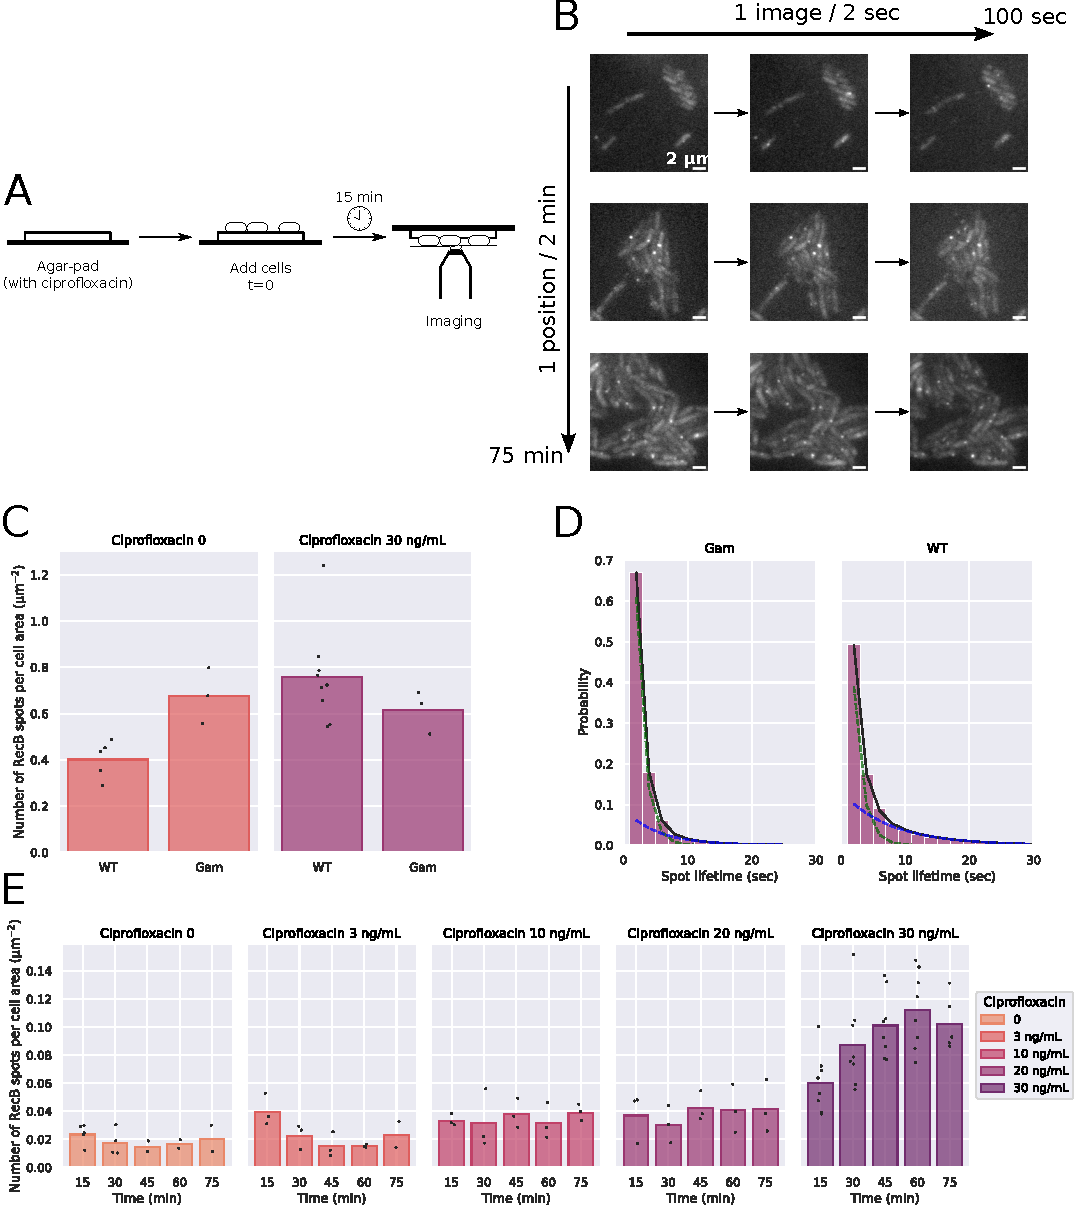
\includegraphics[width=.8\textwidth]{Figures/Fig2_cipro_nSpots.pdf}
    \caption{RecB DNA binding under ciprofloxacin exposure. \textbf{(A)} Example kymographs of RecB throughout an acquisition. A short timelapse (100 sec) is acquired at a different position every 2 min for 75 min. \textbf{(B)} RecB spot lifetime histograms at 3, 10, 20 and 30 ng/mL ciprofloxacin (bars), fitted with a bi-exponential decay model (black line, fit components showed as dashed lines). \textbf{(C)} RecB spot lifetime histograms for cells over-expressing the Gam protein, under 0 or 30 ng/mL ciprofloxacin (bars), fitted with a bi-exponential decay model (black line, fit components showed as dashed lines). \textbf{(D)} Proportion of RecB spots that are shorter than a given lifetime, for cells over-expressing the Gam protein. Black dots show individal datasets, the black line is the average between them, and the red dashed line shows the smallest lifetime at which 95\% of RecB spots are shorter.}
    \label{Fig:lifetime_fits}
\end{figure*}

%% We add ciprofloxacin to increase the level of DNA damage
To gain more insight into DNA binding by RecB, we induced additional DSBs by adding ciprofloxacin to agar pads before imaging. Cells were left to settle down on the pad for 15 min, and then 50-frame timelapse videos were acquired at a rate of one position every 2 min (Figure \ref{Fig:lifetime_fits}A) for 60 min. This allowed us to quantify RecB binding at different time points ranging from 15 to 75 min after ciprofloxacin exposure.

%% RecB spot lifetime histograms change upon exposure to ciprofloxacin
%%% They are not well-fitted by a monoexponential decay (SI fig)
%%% We fit with a bi-exponential decay model
%%% Mention lifetimes/proportions, in table
Upon exposure to ciprofloxacin, the RecB spot lifetime histograms contained more long-lived spots. Fitting with a mono-exponential decay model as in Figure \ref{Fig:endogenous}D did not account well for these long-lived spots (Supp. Figure \ref{SIFig:monoexp_fits}), especially at the higher ciprofloxacin concentrations. This suggested that the new long-lived spots that appeared under exposure to ciprofloxacin corresponded to a new population of RecB spots, that had a slower dissociation rate from DNA than the ones observed under endogenous damage. Indeed, fitting with a bi-exponential decay model ($y = a_1.e^{-k_1.t} + a_2.e^{-k_2.t}$) accounted much better for the longer-lived RecB spots (Figure \ref{Fig:lifetime_fits}B). The bi-exponential fit outlined two populations of spots, with different lifetimes: a short-lived one, with lifetimes ranging from 1.2 to 1.5 sec, and a longer-lived one, with lifetime between 5 and 10 sec (Table \ref{tab:fit_results}). Even though the short-lived spots always represented a majority of events ($>$ 90\% of the spots), the proportion of long-lived spots tended to increase under higher ciprofloxacin exposure (from 3.4\% $\pm$ 0.9 under 3 ng/mL ciprofloxacin to 7.5\% $\pm$ 2 under 30 ng/mL ciprofloxacin).

\begin{table}[htbp]
    \centering
    \begin{tabular}{llll}
        \toprule
         &  & Lifetime (sec) & Proportion (\%) \\
        Ciprofloxacin & Type &  &  \\
        \midrule
        \multirow[t]{2}{*}{0} & Short & 1.24 $\pm$ 0.2 & 97.38 $\pm$ 0.72 \\
         & Long & 7.15 $\pm$ 1.2 & 2.62 $\pm$ 0.72 \\
        \cline{1-4}
        \multirow[t]{2}{*}{3 ng/mL} & Short & 1.17 $\pm$ 0.16 & 96.6 $\pm$ 0.89 \\
         & Long & 5.54 $\pm$ 1.06 & 3.4 $\pm$ 0.89 \\
        \cline{1-4}
        \multirow[t]{2}{*}{10 ng/mL} & Short & 1.18 $\pm$ 0.14 & 94.91 $\pm$ 0.8 \\
         & Long & 6.53 $\pm$ 1.36 & 5.09 $\pm$ 0.8 \\
        \cline{1-4}
        \multirow[t]{2}{*}{20 ng/mL} & Short & 1.39 $\pm$ 0.18 & 95.78 $\pm$ 0.83 \\
         & Long & 9.21 $\pm$ 1.14 & 4.22 $\pm$ 0.83 \\
        \cline{1-4}
        \multirow[t]{2}{*}{30 ng/mL} & Short & 1.49 $\pm$ 0.23 & 92.48 $\pm$ 1.95 \\
         & Long & 9.83 $\pm$ 1.74 & 7.52 $\pm$ 1.95 \\
        \bottomrule
        \end{tabular}
    \caption{Parameters derived from the spot lifetime histogram fits (Figures \ref{Fig:endogenous}D and \ref{Fig:lifetime_fits}B). The lifetime was calculated as the inverse of the fitted dissociation rate. Values are given as the mean $\pm$ standard deviation over 3 independent datasets.}
    \label{tab:fit_results}
\end{table}

%% To check what these two populations are, we use the Gam protein to prevent DNA binding and fit with the same model
%%% Short-lived population stays, long-lived one is removed
%%% Interpretation: because of its size, the RecBCD-Halo-Gam complex can sometimes form spots (SI Note + SI Fig if any), which creates short spots
%%% Therefore, we are unable to detect short DNA binding events, but we can confidently detect longer DNA binding events
To determine whether both short- and long-lived spots resulted from RecB binding to DNA, we measured RecB spots lifetime in the presence and absence of ciprofloxacin while over-expressing the Gam protein of phage $\lambda$ from a plasmid. The Gam protein was previously shown to bind in place of DNA on the RecBCD complex\cite{Wilkinson2016}, and its overexpression is expected to abolish RecBCD binding to DNA. Accordingly, cells that over-expressed Gam and were exposed to high ciprofloxacin (30 ng/mL) showed little elongation compared to cells that did not overexpress Gam (Supp. Figure \ref{SIFig:Gam_cell_length}). The resulting RecB spot lifetime histograms showed a near-complete disappearance of the long-lived spots, while short-lived ones were still present (Figure \ref{SIFig:Gam_RecB_lifetimes_fits}). This was confirmed by fitting the histogram with our bi-exponential decay model, which found proportions of long-lived spots ($\sim$3\%) similar to those in wild-type cells that were not exposed to ciprofloxacin (2.6\%, Table \ref{tab:fit_results}). This confirmed that (i) long-lived RecB spots correspond to RecB molecules that have bound to DNA, and (ii) short-lived RecB spots can result from other causes than short-lived DNA binding (Supp. Note \ref{note:spurious_spots} and Supp. Figure \ref{SIFig:displacement_simul}). Spots that live only for a few seconds cannot be reliably assigned to one or the other category. However, based on the Gam overexpression data, we determined that any spot with a lifetime over 10 sec had 95\% probability to be DNA-bound (Figure \ref{Fig:lifetime_fits}C).

%% We use the number of spots and proportion of long-lived spots to estimate the rate of recruitment of RecB on the DNA (Fig 2D)
%% Mention/link to discussion on relationship between RecB recruitment rate and DSB formation rate
Whereas the lifetime of the fluorescent spots informs us on how long RecB stays bound to DNA, the rate of appearance of spots helps us estimate the rate of recruitment of RecB to DNA under a certain DNA damage condition. To achieve this, we need to quantify for each timelapse the total number of spots that belong to the "long-lived" (i.e. RecB bound to DNA) category. Since the short- and long-lived populations cannot be clearly separated from the lifetime histograms (Figure \ref{Fig:lifetime_fits}B), we have to take an "ensemble-level" approach. For each dataset, multiplying the total number of spots that appear during the timelapse by the proportion of long-lived spots retrieved from the lifetime histogram fits gives us an estimate of the number of DNA-bound RecB per timelapse (Figure \ref{Fig:lifetime_fits}D). We estimate that under endogenous damage and under low ciprofloxacin concentrations, on average 1 to 2 RecB molecules are recruited to the DNA per hour. This is roughly consistent with the previous estimate of 18\% of cells generating an endogenous DSB per cell cycle\cite{Sinha2018} (see discussion). At ciprofloxacin concentrations above the MIC (30 ng/mL), the recruitment rate increases sharply to an average of 5 RecB recruited to DNA per hour. Furthermore, we expect that this recruitment rate gives a close estimate of the rate of formation of DSBs (see discussion).

% Part 3: Effects of DSBs and the repair process on the cell
\subsection*{There are two regimes of DNA repair for ciprofloxacin-induced damage}  % TITLE TO BE CHANGED

\begin{figure*}[htbp]
    \centering
    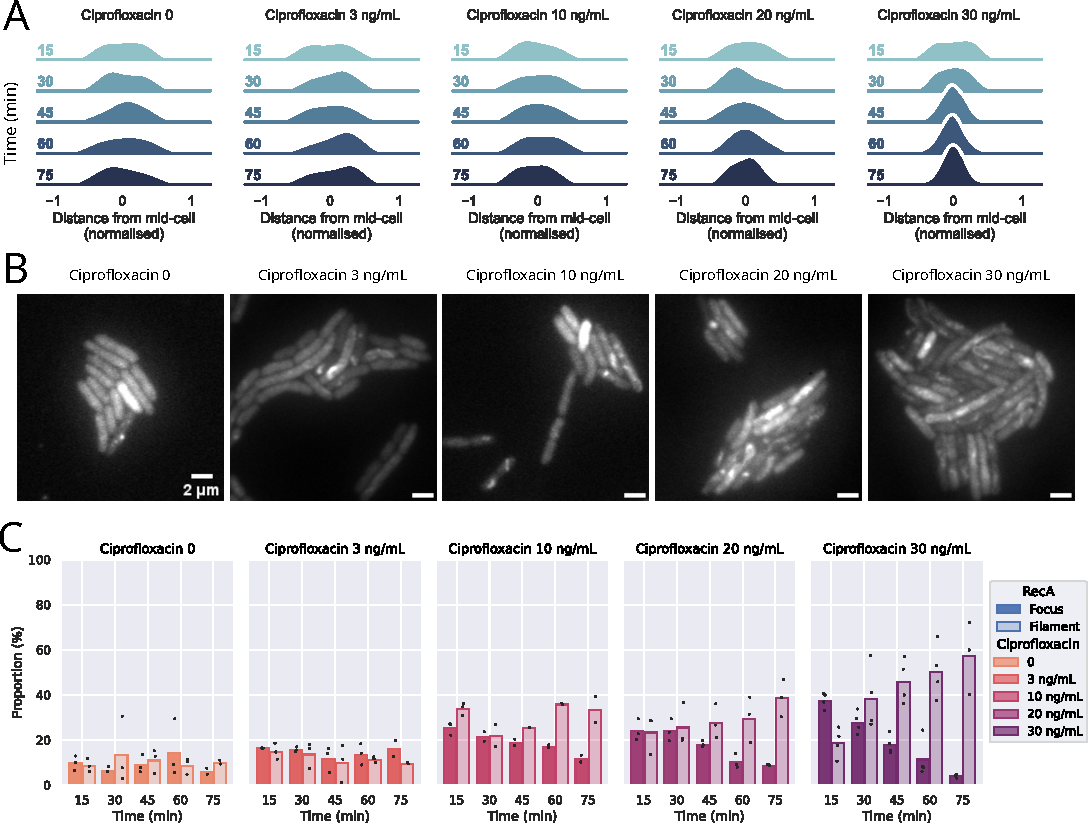
\includegraphics[width=.8\textwidth]{Figures/Fig4_cipro_30ngmL.pdf}
    \caption{Accumulation of DSB repair intermediates under exposure to ciprofloxacin. \textbf{(A)} Number of long-lived ($>$10 sec) RecB spots per cell area. Black dots represent individual datasets, and bars the average between them. \textbf{(B)} Position of long-lived RecB spots along the cell's long axis (normalised). \textbf{(C)} Representative images of cells containing different RecA structures (diffuse fluorescence, foci or filaments). Arrows point to representative examples of each of these structures. \textbf{(D)} Proportion of cells containing RecA foci or filaments. Black dots represent individual datasets, and bars the average between them.}
    \label{Fig:high_cipro}
\end{figure*}

%% We see a strong accumulation of RecA filaments (RecA foci seem to be transient and their number decreases over time)
Upon exposure to the highest cipro\-floxacin concentration (30 ng/mL), RecA filaments became visible in a large number of cells at the higher ciprofloxacin concentrations (Figure \ref{Fig:high_cipro}C). Although the proportion of cells that contained RecA filaments was initially low under all ciprofloxacin concentrations ($<$20\%), after one hour of exposure the proportion of cells that contained a RecA filament had increased to $\sim$40\% at 20 ng/mL ciprofloxacin, and $\sim$60\% at 30 ng/mL (Figure \ref{Fig:high_cipro}D). RecA foci on the other hand seemed to form quickly following ciprofloxacin exposure (present in $\sim$40\% of the cells after 15 min of exposure to 30 ng/mL ciprofloxacin) and come back to endogenous damage level after $\sim$1 hour. Taken together, these results show that RecA foci are transient structures in the repair process that do not accumulate under high DNA damage, whereas RecA filaments do accumulate, presumably when the homologous sequence cannot be found.

%% We imaged nucleoid and RecB in the same experiment
%% We observe the effect of ciprofloxacin exposure on Nucleoid position
%% (fraction of cell occupied by nucleoid in SI)


%% Nucleoid and RecB position are correlated
%% Interpretation: RecB spot centring is due to nucleoid centring (not obvious: link to RecB recruitment rate, explain it happens after several rounds of DSBs)


%% Conclude: there are two regimes of DNA repair for ciprofloxacin-induced damage:
%% 1. Sub-lethal cipro concentrations, where repair structures are formed then disappear as damage gets repaired
%% 2. Lethal concentrations of cipro, where repair structures are formed and accumulate over time while the cell fails to repair its DNA
% (this could be part of a wider conclusion)
We observe two regimes of DNA repair after ciprofloxacin exposure. At sub-MIC ciprofloxacin concentrations (0, 3, 10 ng/mL), repair structures such as RecB spots and RecA filaments form transiently and disappear as the damage gets repaired. At higher ciprofloxacin concentrations (20, 30 ng/mL), the DNA damage caused is more extensive, and repair structures are formed and accumulate over time while the cell fails to repair its DNA, ultimately leading to cell death.

% Part 4: Mutants in the repair pathway
\subsection*{RecB dissociation depends on RecA loading}  % TITLE TO BE CHANGED

\begin{figure*}[htbp]
    \centering
    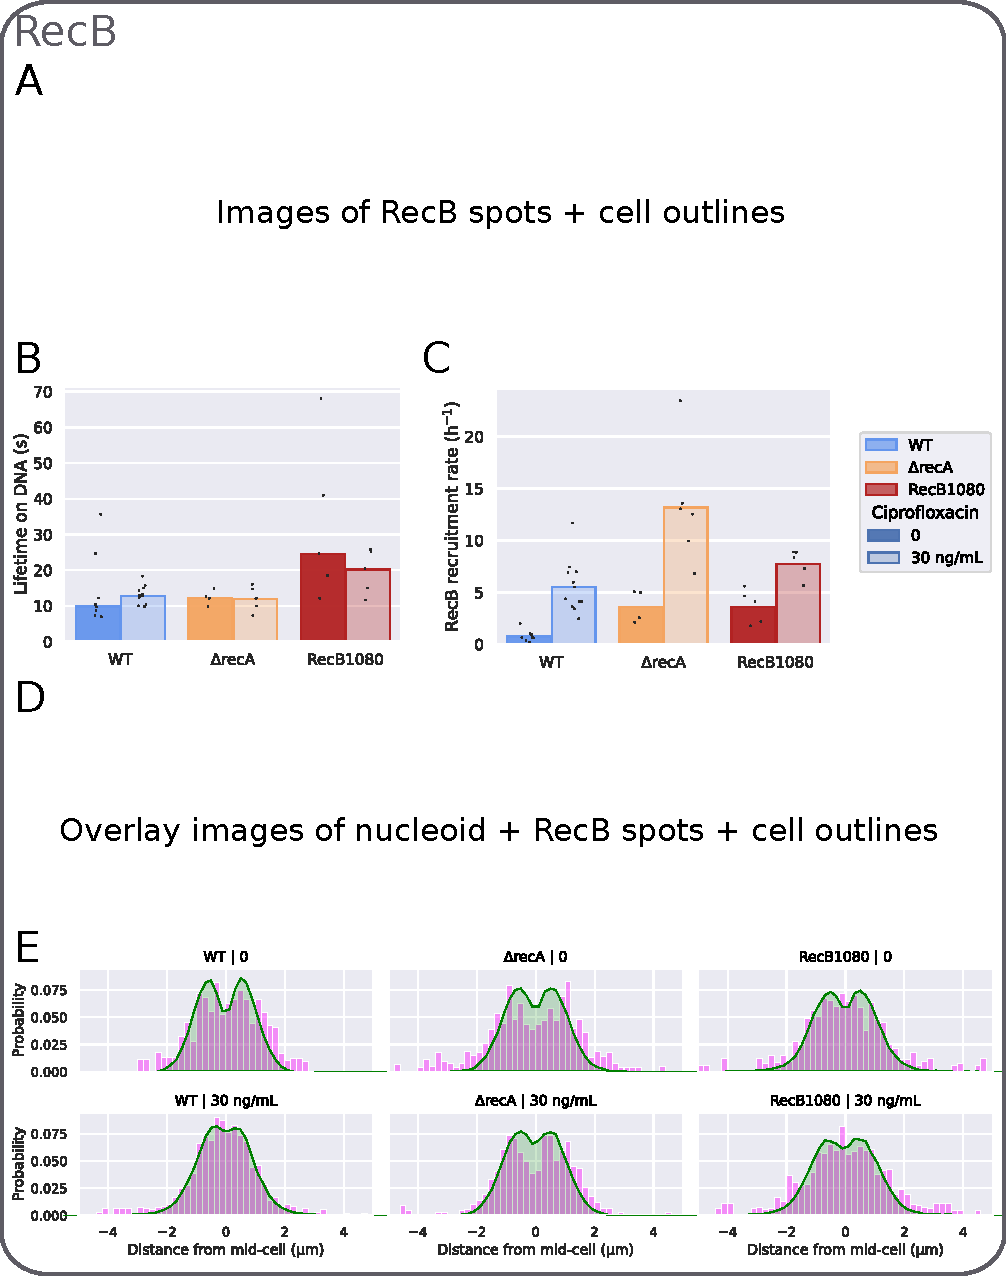
\includegraphics[width=.8\textwidth]{Figures/Fig5_mutants.pdf}
    \caption{RecB binding to DNA (RecB spots with lifetime $>$10 sec) in the \dreca, \teneighty\ and \dreca-\teneighty\ mutant strains. \textbf{(A)} Number of long-lived DNA-bound RecB per cell area. Black dots represent individual datasets, and bars the average between them. \textbf{(B)} Position of long-lived DNA-bound RecB along the cell's long axis (normalised).}
    \label{Fig:mutants}
\end{figure*}

%% Fitting spot lifetime histograms with bi-exponential model
To better understand the factors that contribute to the dissociation of RecB from the DNA, we imaged two different mutants (\dreca\ and \teneighty), in the presence or absence of 30 ng/mL ciprofloxacin. Similarly to the WT, we computed histograms of RecB spot lifetimes, and fitted them with a bi-exponential decay model (Supp. Figure \ref{SIFig:mutants_biexp_fits}), from which we extracted the slower rate, corresponding to the dissociation of DNA-bound RecB molecules. The corresponding lifetimes for DNA-bound RecB are shown on Figure \ref{Fig:mutants}A.

%%% drecA
In the \dreca\ mutant in the absence of ciprofloxacin, the lifetime of DNA-bound RecB is increased compared to the WT strain. This suggests that the formation of a RecA filament on the 3' ssDNA following RecBCD action could contribute to RecBCD dissociation from the DNA. Similarly to the wild-type strain, the lifetime of DNA-bound RecB was slightly increased upon exposure to 30 ng/mL ciprofloxacin.

%%% RecB1080 has even longer lifetime than drecA. This means something else than RecA loading deficiency must make RecB dissociation difficult. We can hypothesise that it's RecB nuclease deficiency, which might make it hard for RecBCD to come off the DNA once it's threaded in
Both in the presence and absence of ciprofloxacin, the \teneighty\ mutant shows more DNA-bound RecB than the WT or the \dreca\ mutant. This suggests that the increased lifetime of \teneighty\ on the DNA is not only due to its deficiency in RecA loading but also to the absence of its nuclease activity. It is possible that unwinding DNA without digesting it makes dissociation more challenging due to the DNA strands threading through the RecBCD complex. Of note, exposure to ciprofloxacin does not increase the DNA-binding lifetime of \teneighty.

%%% Spot lifetime histogram tails are not well fitted by a bi-exponential model (they only represent 1-3% of the spots)
%%% A tri-exponential decay model fits the tail better, and yields a very slow dissociation rate
%%% The very slow rates are ~ equal to bleaching, so the spot lifetime cannot be estimated. However, we know that it's very long
Zooming on the tails of the RecB spot lifetime histograms reveals there is a fraction of very long-lived RecB spots (> 50 sec) which are not well accounted for by our bi-exponential fit. These spots represent 1-3\% of all RecB spots. Even though fitting with a triple-exponential model accounts well for these very long RecB spots, the corresponding spot disappearance rate is extremely close to the bleaching rate. We are therefore not able to precisely determine the lifetime of these very long-lived spots, but we can assume that they are extremely long-lived (on the scale of minutes). These spots might correspond to RecB molecules that are trapped on DNA, in a conformation where they are almost entirely unable to dissociate.

%% RecB spots in ΔrecA and/or 1080 background in the presence of ciprofloxacin are not centred as in WT (to be extended with sytox data)
%%% In ΔrecA there is no centring and even a slight "exclusion" of spots from the centre of the cell. This confirms the involvement of the SOS response in RecB spot centring.
Upon addition of high concentrations of ciprofloxacin (20-30 ng/mL) to wild-type cells, DNA-bound RecB molecules were mainly found in the centre of the cell (Figure \ref{Fig:high_cipro}A), consistently with SOS-dependent compaction of the bacterial chromosome. In the \dreca\ mutant at 30 ng/mL ciprofloxacin, DNA-bound RecB were found throughout the cell, with a slightly lower density towards the centre (Figure \ref{Fig:mutants}B). This pattern is similar to what would be expected of a DNA-bound protein in the absence of chromosome compaction\cite{Stracy2021}. This observation reinforces the idea that the centring of DNA-bound RecB observed in the wild-type under high ciprofloxacin depends on the SOS response.

%%% In 1080 there is no centring, but also no exclusion from the centre of the cell. This might correspond to a "mixed" population, where only a few spots get centred due to the delay in the SOS response
Interestingly, in the \teneighty\ mutant a more even distribution of DNA-bound RecB is observed. The density of bound molecules is not reduced at the centre of the cell, as was observed in the \dreca\ mutant (Figure \ref{Fig:mutants}C). This could be attributed to a significantly delayed chromosome compaction, due to the largely reduced efficiency of RecA loading in the \teneighty\ mutant.

